\documentclass[12pt,a4paper]{article}
%\documentclass[11pt,UTF8]{article}
%\usepackage{ctex}
\usepackage{tcolorbox}
\usepackage{graphicx}
\usepackage{geometry}
\usepackage{listings}
\usepackage{xcolor}
\usepackage{mathtools}
\usepackage{framed} 
\usepackage{amsfonts}
\usepackage{algpseudocode} 
\usepackage{algorithm}
\usepackage{ulem}
\usepackage{tikz}

\renewcommand{\algorithmicrequire}{ \textbf{Input:}} %Use Input in the format of Algorithm
\renewcommand{\algorithmicensure}{ \textbf{Output:}} %Use Output in the format of Algorithm
\definecolor{codegreen}{rgb}{0,0.6,0}
\definecolor{codegray}{rgb}{0.5,0.5,0.5}
\definecolor{codepurple}{rgb}{0.58,0,0.82}
\definecolor{backcolour}{rgb}{0.95,0.95,0.92}

\usepackage{tikz}
\usepackage{tikz-qtree}

\begin{document}
\noindent

%========================================================================
\noindent\framebox[\linewidth]{\shortstack[c]{
\Large{\textbf{Homework 3}}\vspace{1mm}\\
VE216 - Introduction to Signal and Systems, Qiao Heng, Spring 2021}}

\begin{center}

\footnotesize{\color{blue}$*$ Name: Han Yibei \quad Student ID: 519370910123 \quad Email: 1982600614@qq.com}
\end{center}

\section*{HW Notes:}
\begin{itemize}
    \item Problems where the number of points are followed by an exclamation are basic skill problems and will be graded without partial credit.
    \item \fbox{Box} your final answer. You will be graded on both the final answer and the steps leading to it. Correct intermediate steps will help earn partial credit.
    For full credit, \sout{cross out} any incorrect intermediate step.
    \item If you need to make any additional assumptions, state them clearly.
    \item Legible writing will help when it comes to partial credit.
    \item Simplify your result when possible.
\end{itemize}

\newpage
\section*{Problems:}
\normalsize
\begin{tcolorbox}[colback = white]
1. [15!]Find the Fourier series representations of the following signals. Express your answer in a real form.\\
(a) $x(t)=\sum_{n=-\infty}^{\infty}\delta(t-3n)$\\
(b) $x(t)=\sum_{n=-\infty}^{\infty}rect(\frac{-t-5n+3}{6})$\\
(c) The signal illustrated below,
\begin{center}
    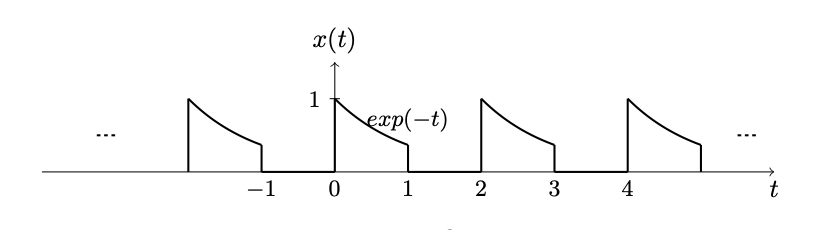
\includegraphics[scale=0.4]{p1(c).png}
\end{center}
\end{tcolorbox}

\begin{tcolorbox}
\normalsize
\textcolor{blue}{Solution:\\
(a) $T=3\qquad \omega=\frac{2\pi}{T}=\frac{2\pi}{3}$ \\
\begin{equation*}
    \begin{aligned}
        c_k=\frac{1}{3}\int_{1}^{4}\delta(t-3)e^{-jk\frac{2\pi}{3}t}dt=\frac{1}{3}
    \end{aligned}
\end{equation*}
\begin{equation*}
    \begin{aligned}
        x(t)&=\sum_{k=-\infty}^\infty\frac{1}{3}e^{jk\frac{2\pi}{3}t}\\
        &\fbox{$=\frac{1}{3}+\frac{2}{3}\sum_{k=1}^\infty cos(k\frac{2\pi}{3}t)$}
    \end{aligned}
\end{equation*}
(b) $T_0=5~~\omega_0=\frac{2\pi}{5}=\frac{2\pi}{5}$\\
And we can get $x(t)=c_0+\sum_{k=1}^\infty (a_k cos(k\omega t)+b_k sin(k\omega t))$\\
$$
c_{0}=\frac{1}{T} \int_{T_{0}} x(t) d t=\frac{6}{5}
$$
And for $k \in \mathbb{Z}^{+}$
$$
\begin{aligned}
a_{k} &=\frac{2}{T} \int_{T_{0}} x(t) \cos (k \omega t) d t \\
&=\frac{2}{T}\left(\int_{0}^{1} 2 \cos (k \omega t) d t+\int_{1}^{5} \cos (k \omega t) d t\right) \\
&=\frac{1}{k \pi}(\sin (5 k \frac{2\pi}{5})+\sin (k \frac{2\pi}{5})) \\
&=\frac{1}{k \pi} sin(\frac{2\pi k}{5})
%&=\frac{1}{k \pi}\left(1-\cos \left(\frac{2 \pi k}{5}\right)\right)
\end{aligned}
$$
$$
\begin{aligned}
b_{k} &=\frac{2}{T} \int_{T_{0}} x(t) \sin (k \omega t) d t \\
&=\frac{2}{T}\left(\int_{0}^{1} 2 \sin (k \omega t) d x+\int_{1}^{5} \sin (k \omega t) d x\right) \\
&=\frac{1}{k \pi}(2-\cos (k \omega)-\cos (5 k \omega)) \\
&=\frac{1}{k \pi}(1-\cos(\frac{2 \pi k}{5}))
\end{aligned}
$$
Therefore, from the equations above, we can conclude that
$$\fbox{$
x(t)=\frac{6}{5}+\frac{1}{\pi} \sum_{k=1}^{\infty}\frac{1}{k}[sin(\frac{2\pi k}{5}) cos(\frac {2\pi kt}{5})+(1-\cos(\frac {2 \pi k}{5}))sin(\frac{2\pi kt}{5})]
$}$$
}
\end{tcolorbox}

\begin{tcolorbox}
\normalsize
\textcolor{blue}{
(c)$T=2\qquad \omega=\frac{2\pi}{2}=\pi$\\
$x(t)=c_0+\sum_{k=1}^\infty (a_k cos(k\omega t)+b_k sin(k\omega t))$\\
And $c_0=\frac{1}{T} \int_{T_0} x(t) dx=\int_0^1 e^{-t} dt=1-\frac{1}{e}$
$$
\begin{aligned}
    a_{k} &=\frac{2}{T} \int_{T_{0}} x(t) cos (k \omega t) d t\\
    &= \int_0^1 e^{-t} cos (k\pi t) d x\\
    &= \frac{e-(-1)^{k}}{e\left(1+k^{2} \pi^{2}\right)}
\end{aligned}
$$
$$
\begin{aligned}
    b_{k} &=\frac{2}{T} \int_{T_{0}} x(t) sin (k \omega t) d t\\
    &= \int_0^1 e^{-t} sin (k\pi t) d x\\
    &= \frac{k \pi\left(e-(-1)^{k}\right)}{e\left(1+k^{2} \pi^{2}\right)}
\end{aligned}
$$
$$\fbox{$
x(t)=\frac{e-1}{2e}+\frac{1}{e} \sum_{k=1}^{\infty} \frac{e-(-1)^{k}}{1+k^{2} \pi^{2}}(\cos (k \pi t)+k \pi \sin (k \pi t))$}
$$
}
\end{tcolorbox}

\begin{tcolorbox}[colback = white]
2. [10!] We know that for a CT period signal x(t) with $\omega_0=\frac{2\pi}{T}$, and its Fourier series can be represented as,
$$x(t)=\sum_{k=-\infty}^{\infty}a_k e^{j k\omega_0t}$$
$$a_k=\frac{1}{T}\int_0^Tx(t)e^{-jk\omega_0t}dt$$
Show that it can also be expressed in real form as,
$$x(t)=B[0] +\sum_{k=1}^\infty B[k]\cos{(k\omega_0t)}+A[k]\sin{(k\omega_0t)}$$
Where,
$$ \left\{
\begin{aligned}
B[0] & = & \frac{1}{T}\int_0^T x(t)dt \\
B[k] & = & \frac{2}{T}\int_0^T x(t)\cos{(k\omega_0t)}dt \\
A[k] & = & \frac{2}{T}\int_0^T x(t)\sin{(k\omega_0t)}dt
\end{aligned}
\right.
$$
\end{tcolorbox}

\begin{tcolorbox}
\normalsize
\textcolor{blue}{Solution:\\
$$
\begin{aligned}
    x_t=&\sum_{k=-\infty}^{\infty}a_k e^{j k\omega_0t}\\
    =&a0+\sum_{k=1}^{\infty}a_k e^{j k\omega_0t}+a_{-k} e^{-j k\omega_0t}\\
    =&\frac{1}{T}\int_0^T x(t)dt+\sum_{k=1}^{\infty}[\frac{1}{T}\int_0^Tx(t)e^{-jk\omega_0t}dt~e^{j k\omega_0t}+\frac{1}{T}\int_0^Tx(t)e^{jk\omega_0t}dt~e^{-j k\omega_0t}]\\
    =&\frac{1}{T}\int_0^T x(t)dt+\sum_{k=1}^{\infty}[\frac{1}{T}\int_0^Tx(t)(cos(-k\omega_0 t)+sin(-k\omega_0 t))dt~e^{j k\omega_0t}\\
    &+\frac{1}{T}\int_0^Tx(t)(cos(k\omega_0 t)+sin(k\omega_0 t))dt~e^{-j k\omega_0t}]\\
    =&\frac{1}{T}\int_0^T x(t)dt +\sum_{k=1}^\infty \frac{2}{T}\int_0^T x(t)\cos{(k\omega_0t)}dt\cos{(k\omega_0t)}\\
    &+\frac{2}{T}\int_0^T x(t)\sin{(k\omega_0t)}\sin{(k\omega_0t)}
\end{aligned}
$$
So we can get that $x(t)=B[0] +\sum_{k=1}^\infty B[k]\cos{(k\omega_0t)}+A[k]\sin{(k\omega_0t)}$ and
$$ \left\{
\begin{aligned}
B[0] & = & \frac{1}{T}\int_0^T x(t)dt \\
B[k] & = & \frac{2}{T}\int_0^T x(t)\cos{(k\omega_0t)}dt \\
A[k] & = & \frac{2}{T}\int_0^T x(t)\sin{(k\omega_0t)}dt
\end{aligned}
\right.
$$
}
\end{tcolorbox}


\begin{tcolorbox}[colback = white]
3. [15!] Let x(t) be a period signal whose Fourier series coefficient are\\
$$ a_k=\left\{
\begin{array}{rcl}
2 & & ,k=0\\
j(\frac{1}{2})^{|k|}& &,otherwise
\end{array} \right.
$$
Use Fourier series properties to answer the following questions:(The table is on page 206 of your textbook)\\
(a) Is x(t) real?\\
(b) Is x(t) even?\\
(c) Is dx(t)/dt even?
\end{tcolorbox}

\begin{tcolorbox}
\normalsize
\textcolor{blue}{Solution:\\
(a) \fbox{Not real.} Because $a_{-k}\neq a_k^*$\\
(b) \fbox{Even.} Because $a_k=a_{-k}$\\
(c) \fbox{Not even.} Let us assume $b_k$ is the fourier coefficient of dx(t)/dt\\
$$
b_k=j\omega k a_k=-\omega k (1/2)^{|k|}
$$
$b_k\neq b_{-k}$ so it is not even
}
\end{tcolorbox}

\begin{tcolorbox}[colback = white]
4.  [10!] A continuous-time signal x(t) with period T is said to be odd harmonic if in its Fourier series representation\\
$$x(t)=\sum_{-\infty}^{\infty}a_ke^{jk(2\pi/T)t}$$
$a_k=0$ for every non-zero even integer k.\\
(a) Show that if x(t) is odd harmonic, then\\
$$x(t)=-x(t+\frac{T}{2})$$
(b) Show that if x(t) satisfies the relation in (a), then it is odd harmonic.
\end{tcolorbox}
\begin{tcolorbox}
\normalsize
\textcolor{blue}{Solution:\\
(a)
\begin{equation*}
    \begin{aligned}
        -x(t+\frac{T}{2})=&-\sum_{-\infty}^{\infty}a_ke^{jk\omega(t+\frac{T}{2})}\\
        =&-\sum_{-\infty}^{\infty}a_k(cos(k\omega(t+\frac{T}{2}))+sin(jk\omega(t+\frac{T}{2})))\\
        =&\sum_{-\infty}^{\infty}a_k(cos(k\omega t)+sin(jk\omega t))\\
        =&\sum_{-\infty}^{\infty}a_ke^{jk\omega(t)}=x(t)
    \end{aligned}
\end{equation*}
(b) $$
\begin{aligned}
a_{k} &=\frac{1}{T} \int_{0}^{T} x(t) \cdot e^{-j k \omega t} d t \\
&=\frac{1}{T} \int_{0}^{\frac{T}{2}}\left(x(t) \cdot e^{-j k \omega t}+x\left(t+\frac{T}{2}\right) \cdot e^{-j k \omega t} \cdot e^{-j k \pi}\right) d t \\
&=\frac{1}{T} \int_{0}^{\frac{T}{2}}\left(x(t)+x\left(t+\frac{T}{2}\right) \cdot e^{-j k \pi}\right) \cdot e^{-j k \omega t} d t\\
&=\frac{1}{T} \int_{0}^{\frac{T}{2}}\left(x(t)+x\left(t+\frac{T}{2}\right)\right) \cdot e^{-j k \omega t} d t \text{(k is integer)}\\
&=\frac{1}{T} \int_{0}^{\frac{T}{2}} 0 d t=0
\end{aligned}
$$     
}
\end{tcolorbox}
\begin{tcolorbox}[colback = white]
5. Consider a casual LTI system realized by the RLC circuit shown below. $x(t)$ is the voltage input (V) and y(t) is the voltage (V) across the capacitor.\\
\begin{center}
    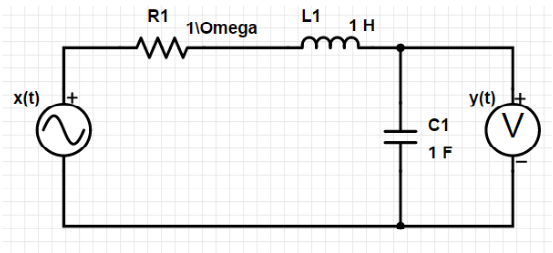
\includegraphics[scale=0.5]{p5.png}
\end{center}
(a) [3!] Find the differential equation relating $x(t)$ and $y(t)$.\\
(b) [3!] Find the system's response to $x(t)=e^{j\omega t}$, where $\omega$ is arbitrary.\\
(c) [1!] Write out the system's transfer function $H(s)$.\\
(d) [1!] Calculate the magnitude of the system's frequency response $|H(j\omega)|$ and plot it as a function of $\omega$.\\
(e) [3!] Use Matlab \textbf{freqs} to generate the exact same plot as part (d). Note that you want to \textbf{plot} the output argument of \textbf{freqs} because directly calling \textbf{freqs} with no output arguments will 1. give two figures; 2. plot both the magnitude and phase response in its default loglog scale. Besides, be sure to specify an appropriate range for the third input argument of \textbf{freqs} using linspace.\\
(f) [3!] Find the Fourier series expansion (in complex exponential form) for $x(t)=1+sin(t)+sin(4t)$ and plot its power density spectrum (by using \textbf{stem}).\\
(g) [2!] Use $x(t)$ as an example to verify Parseval's relation. You may want to use Matlab/Mathematica to calculate (integrate) the power of $x(t)$.\\
(h) [2!] Find the systems output $y(t)$ due to $x(t)$. Plot the power density spectrum of $y(t)$.\\
(i) [2!] Compare $x(t)$ and y(t) and their power density spectrums. What frequency component of the $x(t)$ is attenuated? Is this RLC circuit a lowpass/highpass/bandpass/bandstop filter?
\end{tcolorbox}
\begin{tcolorbox}
\normalsize
\textcolor{blue}{Solution:\\
(a) $$\begin{aligned}
    &C\frac{dy(t)}{dt}=I(t)\\
    x(t)-&R\frac{dy(t)}{dt}-L\frac{dy^2(t)}{dt^2}-y(t)=0\\
    &\fbox{$\frac{d^2y}{dt^2}+\frac{dy}{dt}+y=x$}
\end{aligned}$$
(b)$y(t)=Ae^{j\omega t}$ according to the characteristic of LTI
$$-A\omega^2e^{j\omega t}+A\omega je^{j\omega t}+Ae^{j\omega t}=0$$
$$\Rightarrow A=\frac{1}{1+\omega j-\omega^2}\Rightarrow \fbox{$y=\frac{e^{j\omega t}}{1+\omega j-\omega^2}$}$$
(c)\fbox{$H(s)=\frac{1}{1+s-s^2}$}\\
(d)$|H(j\omega)|=|\frac{1}{1-\omega^2+j\omega}|=\frac{1}{|1-\omega^2+j\omega|}=\fbox{$\frac{1}{\sqrt{\omega^4-\omega^2+1}}$}$
\begin{figure}[H]
    \centering
    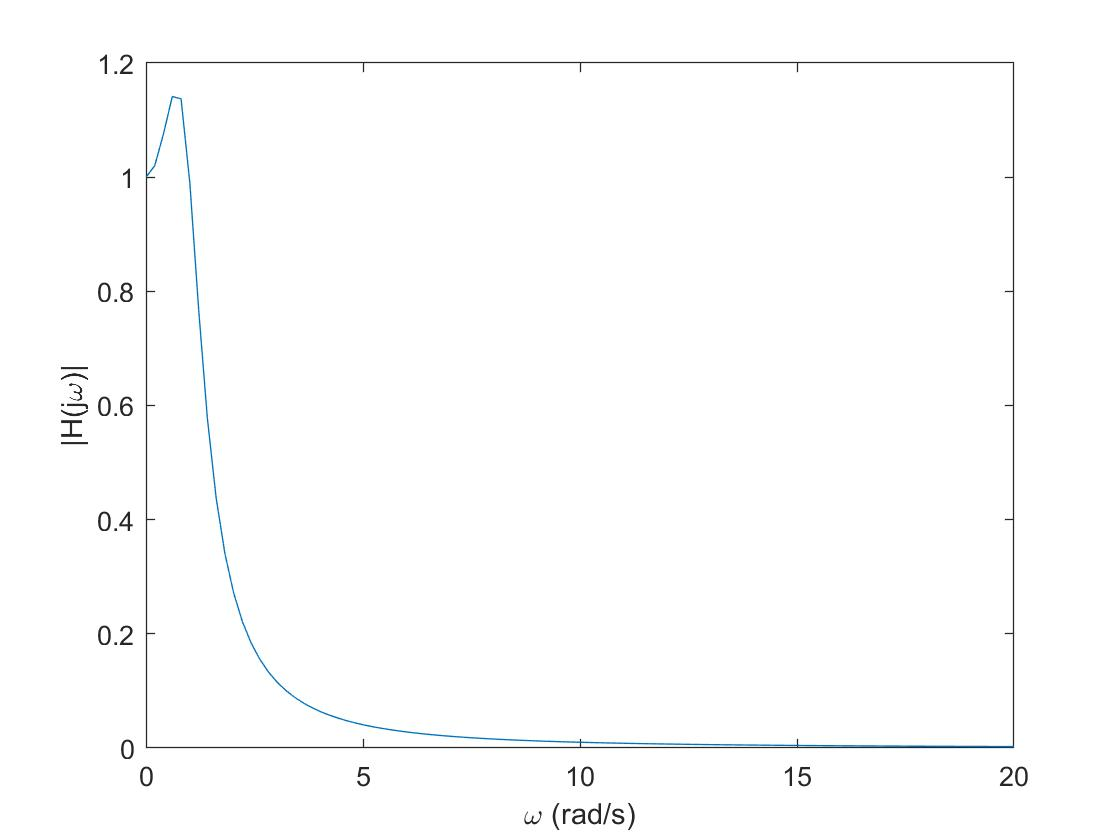
\includegraphics[width=8cm]{5e.jpg}
\end{figure}
(e) \begin{figure}[H]
    \centering
    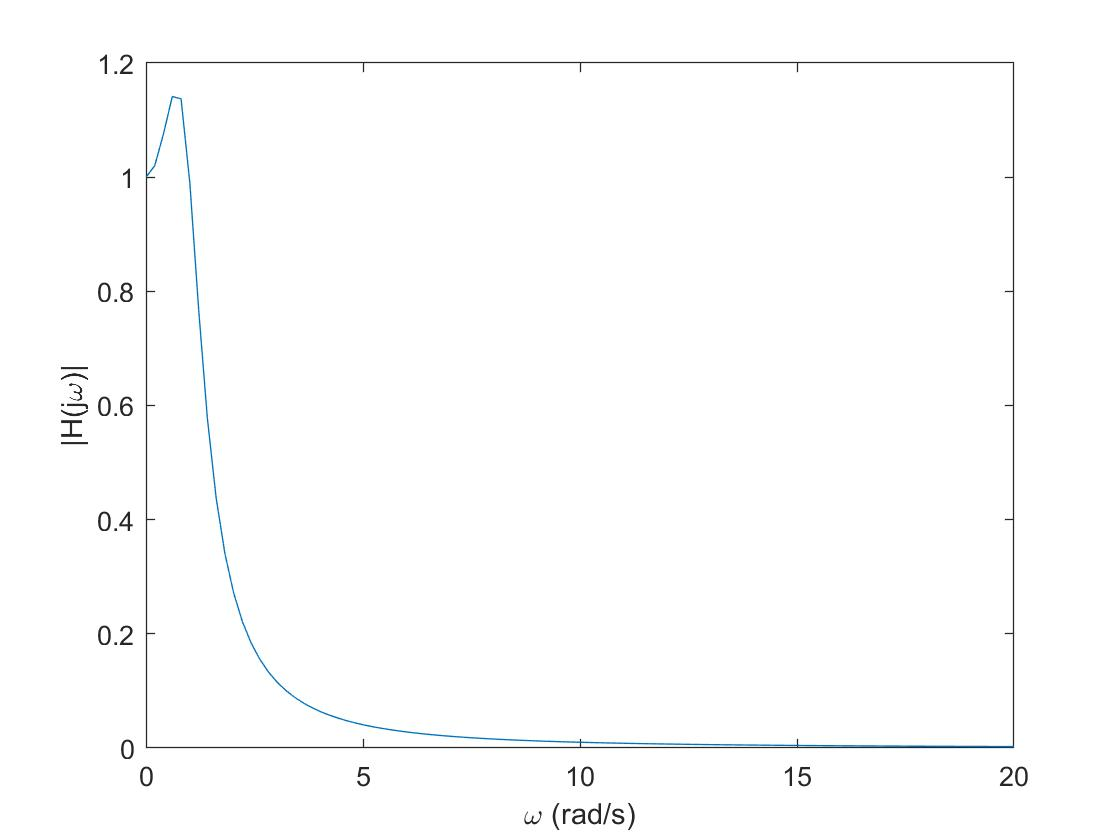
\includegraphics[width=8cm]{5e.jpg}
\end{figure}
}
\end{tcolorbox}

\begin{tcolorbox}
\normalsize
\textcolor{blue}{Solution:\\
(f) \fbox{$x(t)=-\frac{1}{2j}e^{-4jt}-\frac{1}{2j}e^{-jt}+1+\frac{1}{2j}e^{jt}+\frac{1}{2j}e^{4jt}$}
\begin{figure}[H]
    \centering
    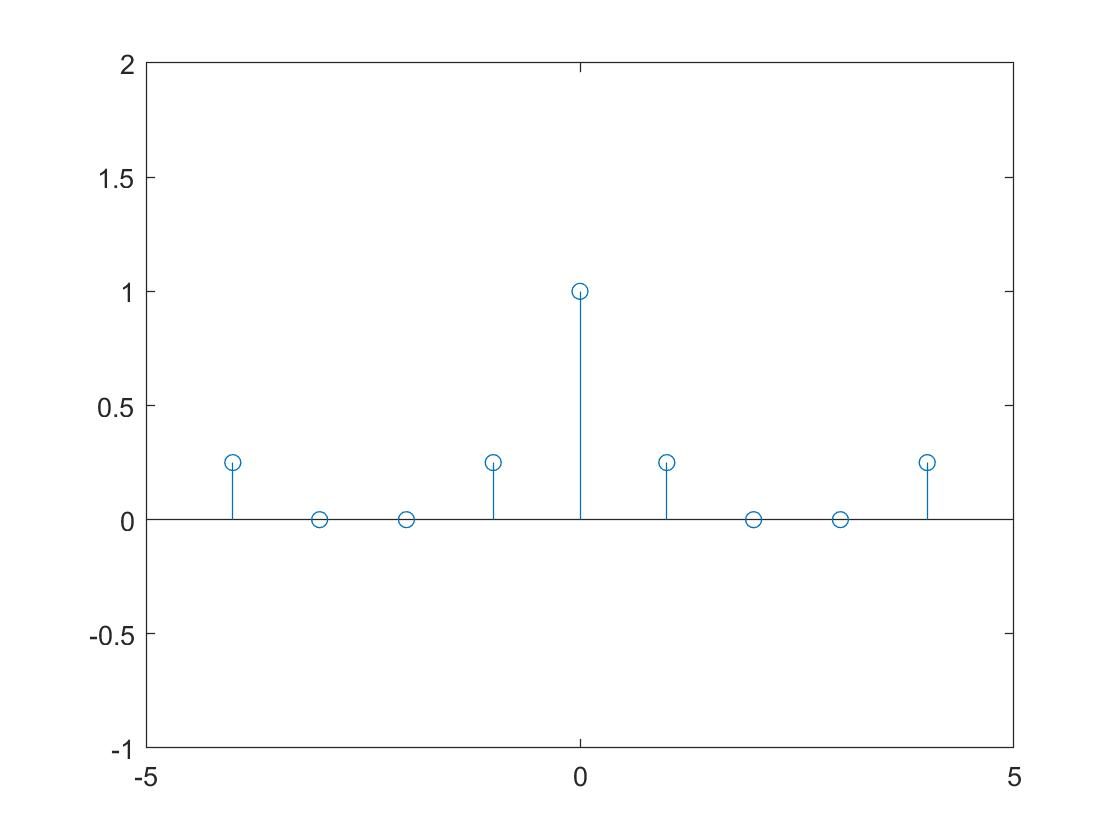
\includegraphics[width=8cm]{5f.jpg}
\end{figure}
(g) $P=\frac{1}{T_0}\int_{T_0}|x(t)|^2dt=\frac{1}{2\pi}\int_{-\pi}^\pi |1+sin(t)+sin(4t)|^2dt=2$\\
$\sum_{k=-\infty}^\infty|c_k|^2=2$, so we can verify the Parseval's relation\\
(h)
$ y(t)=\frac{1}{-\omega^{2}+j \omega+1} x(t)$\\
$H(j)=\frac{1}{j}=-j~~~~ \frac{1}{2 j} H(j)=-\frac{1}{2}$\\
so when $\omega=1$, we have $|c_{k}|^{2}=\frac{1}{4}$, $\omega=-1$, $|c_{k}|^{2}=\frac{1}{4}$, $\omega=\pm 4$, $|c_{k}|^{2}=\frac{1}{964}$
\begin{figure}[H]
    \centering
    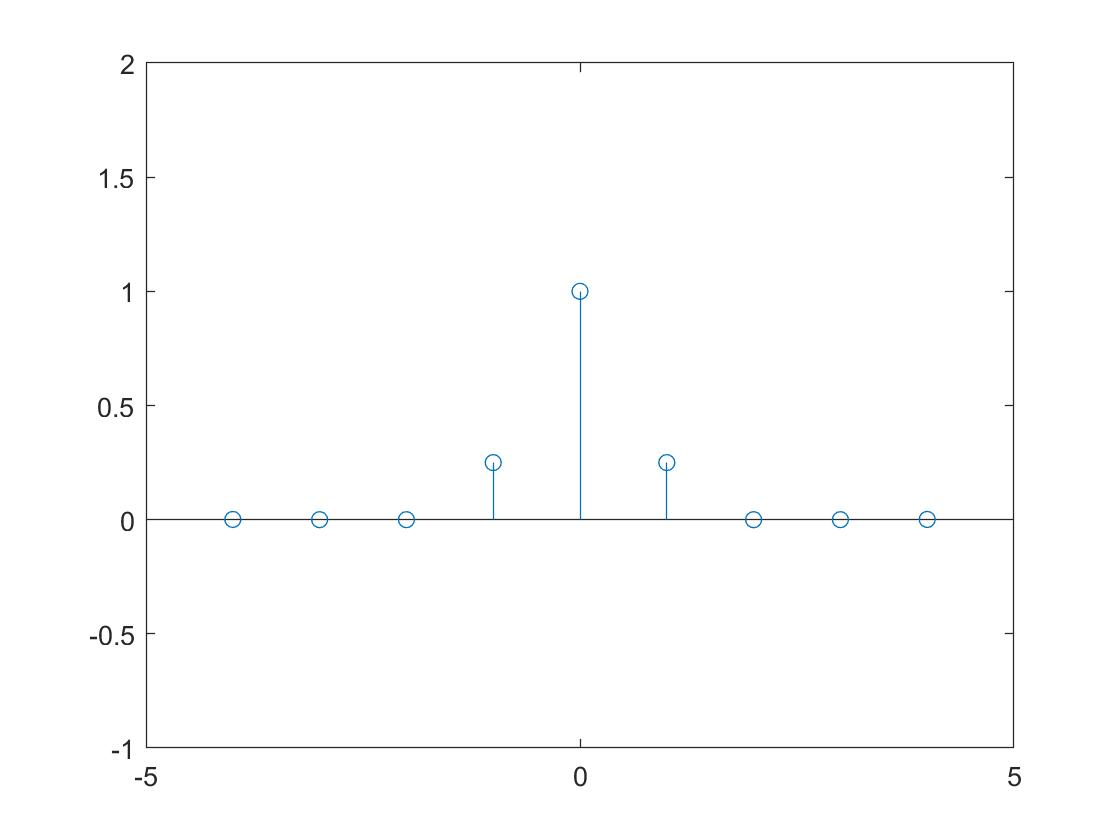
\includegraphics[width=8cm]{5h.jpg}
\end{figure}
(i) The high frequency components of x(t) are smaller \fbox{lowpass filter}
}
\end{tcolorbox}

\begin{tcolorbox}[colback = white]
6. [15!] The Bessel lowpass filter is a widely-used analog linear filter.\\
(a) Make a specific Bessel filter by using Matlab command  \textbf{[num, den]=besself(5,1e4)}, where the two vectors  \textbf{num} and  \textbf{den} are the filter's transfer function's coefficients on the numerator and denominator, respectively. Similar to Problem 5(e), plot the filter's magnitude response from 0 to 20000 rad/s using  \textbf{freqs}.\\
(b) Use Matlab  \textbf{gensig} to generate a square wave with period 0.002 seconds, duration 1 second, and sampling every $10^{-4}$ second. Plot an appropriate portion of the generated signal with axis command.\\
(c) Use Matlab  \textbf{tf} and \textbf{lsim} to simulate the response (output) of the filter to the square wave. Plot your output signal with the same axis range as (b). Compare your input and output. As you can see, the "corners" of the square wave are all "filtered", implying that these corners actually correspond to the high-frequency components of the signal. This also makes sense intuitively as the corners are where the signal change "abruptly".
\end{tcolorbox}

\begin{tcolorbox}
\normalsize
\textcolor{blue}{Solution:}\\
(a)\begin{figure}[H]
    \centering
    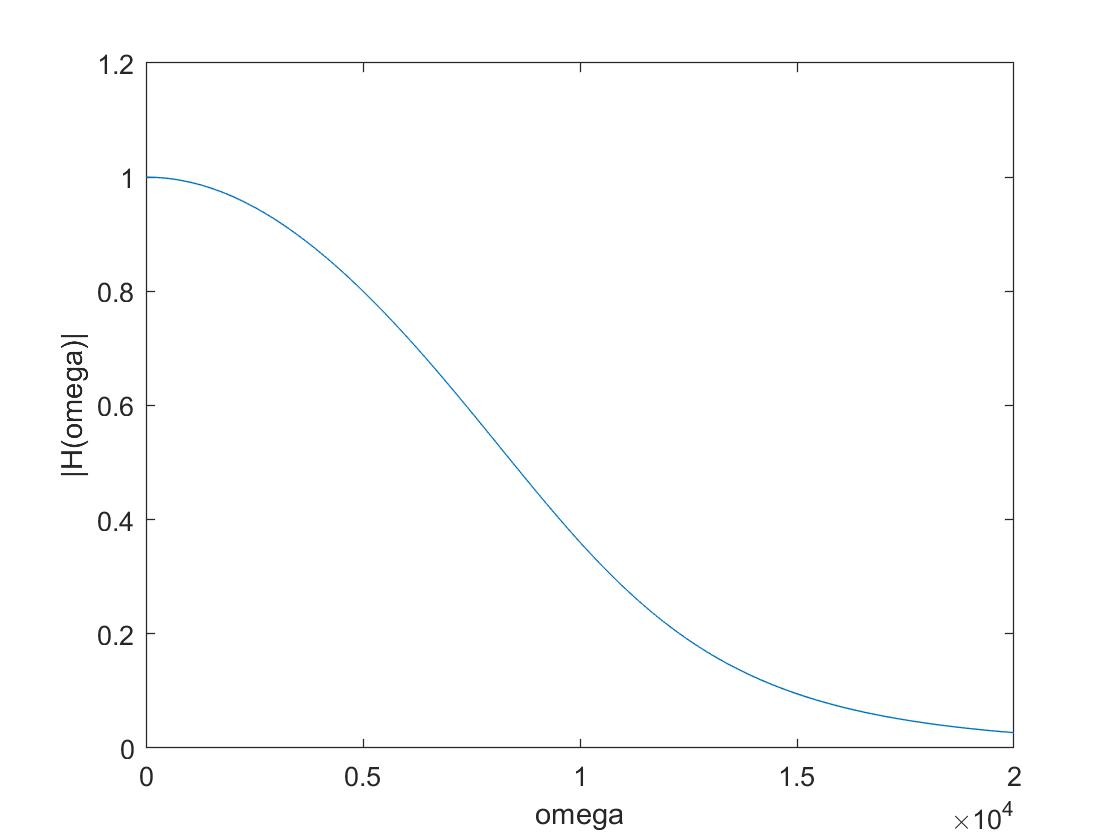
\includegraphics[width=8cm]{6a.jpg}
\end{figure}
(b)\begin{figure}[H]
    \centering
    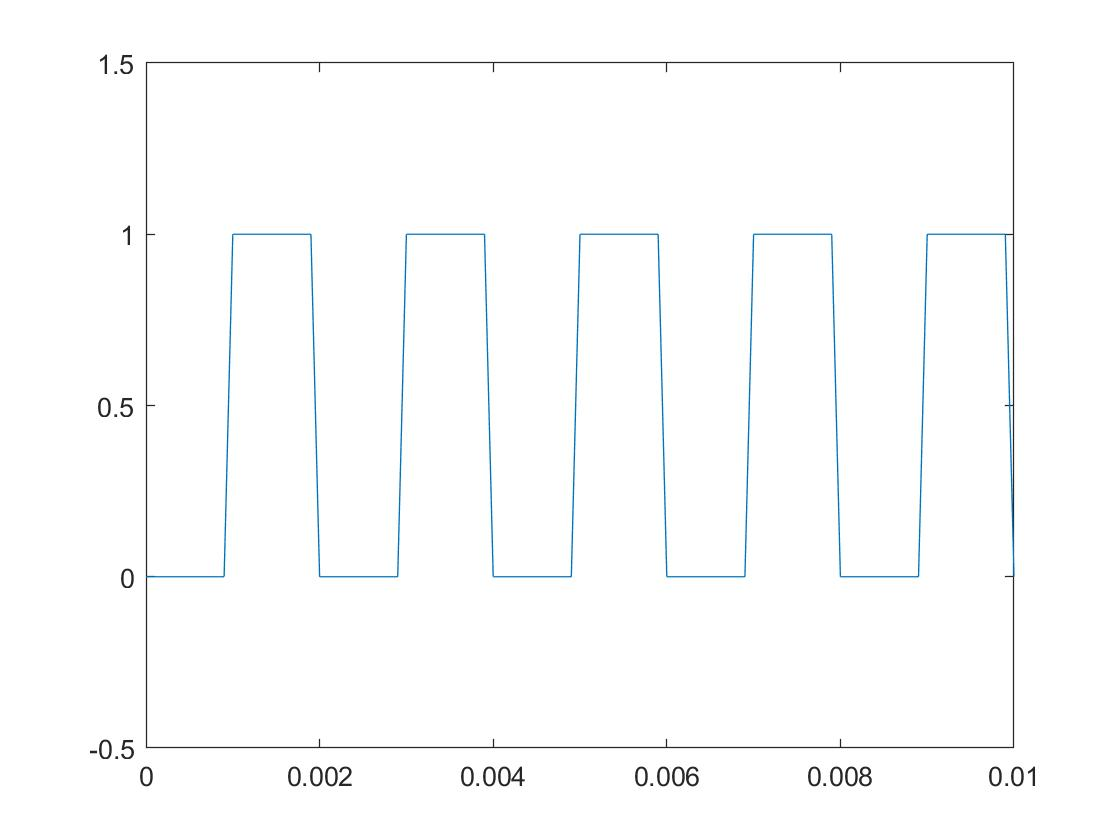
\includegraphics[width=8cm]{6b.jpg}
\end{figure}
(c)\begin{figure}[H]
    \centering
    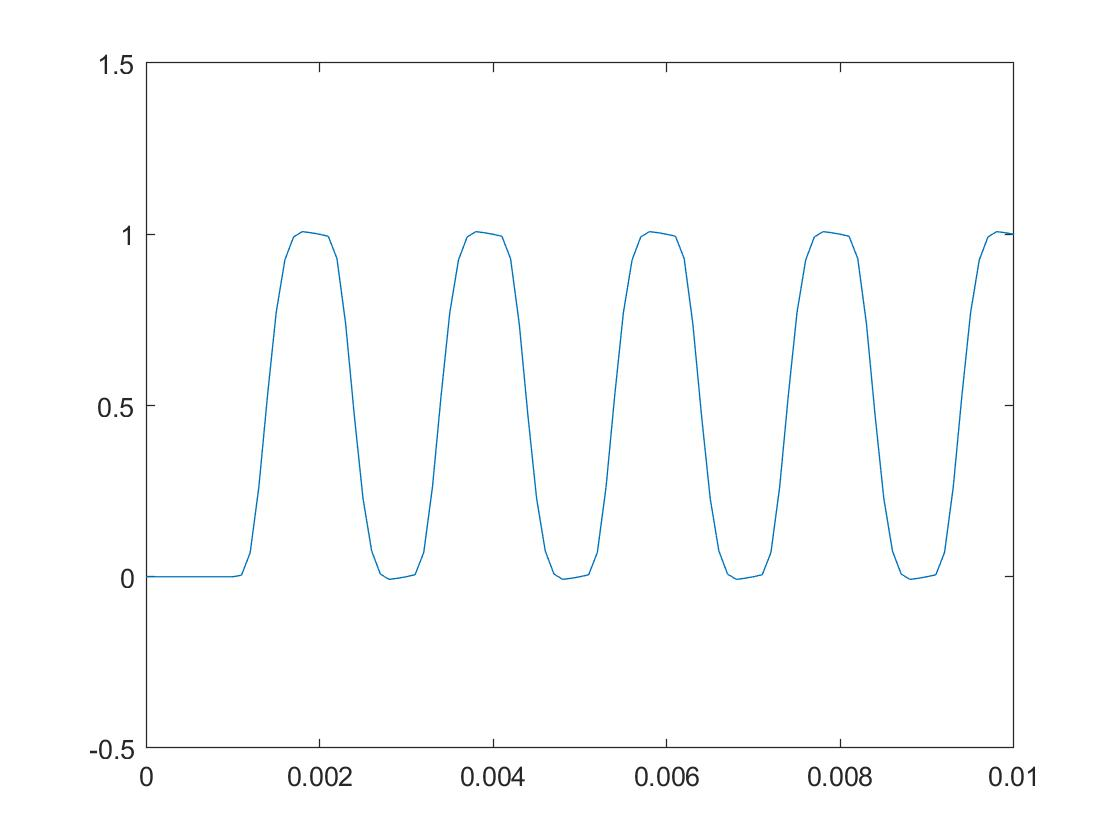
\includegraphics[width=8cm]{6c.jpg}
\end{figure}
\end{tcolorbox}

\begin{tcolorbox}[colback = white]
7. [5!] Assume $x(t)$ is a periodic CT signal with period $T$. Its Fourier series coefficients $a_k$ also have a period $N$. Show that there exist a periodic sequence $g[n]$, so that $x(t)$ is represented by
\begin{center}
    x(t)=$\Sigma_{k=-\infty}^{k=\infty}g[k]\delta(t-kT/N)$.
\end{center}
This means any $x(t)$ with such property actually looks more like a discrete-time signal. This problem shows that typical periodic CT signals will have non-periodic Fourier coefficients.
\end{tcolorbox}
\begin{tcolorbox}
\normalsize
\textcolor{blue}{Solution:\\
\begin{equation*}
    \begin{aligned}
        x(t)=&\sum_{-\infty}^\infty a_k e^{j\frac{2\pi}{T}kt}\\
        =&\sum_{-\infty}^\infty \sum_{k=0}^N a_k e^{j\frac{2\pi}{T}(k+mN)t}\\
        =&\sum_{m=-\infty}^\infty e^{j\frac{2\pi}{T}mNt}\sum_{k=0}^N a_ke^{j\frac{2\pi}{T}kt}\\
        =&\frac{T}{N}\sum_{k=-\infty}^\infty \delta(t-\frac{T}{N}k)\sum_{k=0}^N a_k e^{j\frac{2\pi}{T}kt}\\
        =&\frac{T}{N}\sum_{k=-\infty}^\infty \delta(t-\frac{T}{N}k)g[k]\\
        g[k]=&\fbox{$\sum_{k=0}^N a_k e^{j\frac{2\pi}{T}kt}$}\\
        &\text{ This is a period function with period equal to N}
    \end{aligned}
\end{equation*}
}
\end{tcolorbox}

\begin{tcolorbox}[colback = white]
8 [10!] A distortion present in all amplifiers is in some form of non-linearity. Non-linearities introduce additional frequency components, transferring some of the signal power from the fundamental frequency component to higher harmonics. This is called \textbf{harmonic distortion}. The quality of an amplifier is (in part) judged by how small its \textbf{total harmonic distortion (THD)} is, defined by:
\begin{center}
    THD=$\frac{\mbox{power in DC \& harmonics}}{\mbox{total power}}\cdot 100\%=[1-\frac{\mbox{power in fundamental}}{\mbox{total power}}] \cdot 100\%$.
\end{center}
Consider the following model for an amplifier:
\begin{center}
$y(t)=7[x(t)+bx^5(t)]$
\end{center}
where $b=0.10.$ (This is not a great amplifier). Find the THD for this amplifier, when the input signal is $x(t)=sin(3t)$.
\end{tcolorbox}

\begin{tcolorbox}
\normalsize
\textcolor{blue}{Solution:\\
$sin(3t)=\frac{e^{-j3t}-e^{j3t}}{2j}\Rightarrow sin^5(3t)=\frac{e^{-j15t}-5e^{-j9t}+10e^{-j3t}-10e^{j3t}+5e^{j9t}-e^{j15t}}{j32}$\\
$y(t)=\frac{7[b(e^{-j15t}-e^{j15t})-5b(e^{j9}-e^{-j9})+(16+10b)(e^{-j3t}-e^{j3t})]}{j32}$\\
$|c_{\pm 1}|=\frac{b^2+(5b)^2}{b^2+(5b)^2+(16+10b)^2}\approx \fbox{0.09\%}$
}
\end{tcolorbox}

%========================================================================
\end{document}